\section{Anotações importantes da observação}

\subsection{Os primeiros vídeos}

O primeiro vídeo data de 09/MAI/2014, link \url{https://www.youtube.com/watch?v=8xyller_i5w}, ela com 12 anos ensinando a fazer caixas de doces decoradas, como denuncia a tag \#DIY\footnote{acrônimo de Do it Yourself, faça você mesmo} de Faça Você Mesmo. O vídeo é curto e demonstra que a menina possui desenvoltura e a mesma não se intimida pela câmera. A desenvoltura com que a mesma faz a caixa de doce sugere que ela já lida com trabalhos manuais com muita frequência.

Seguem-se outros vídeos com mesma temática de faça você mesmo, além de experimentação de guloseimas. Num deles faz um react\footnote{react é o termo usados pelos youtubers para reagir a algum fato pela primeira vez} de um unboxing de guloseimas comprados no bairro oriental da Liberdade em SP (\url{https://www.youtube.com/watch?v=qrBjcxeDKJE}). Ela dedica vários vídeos de doces orientais, incluindo os gravados com a mãe.

Nítido notar que a Zabetta é uma menina no final da puberdade, com feições infantis encontrados em qualquer menina da sua idade.

Ela mostra que já tem um time de coração, o Palmeiras, o que demonstra no vídeo \url{https://www.youtube.com/watch?v=W_LVN3bIKqo}, pena que não tem bastidores do pós-jogo para verificar as reações.

Durante um bom tempo ela se dedicou a vídeos de faça você mesma, muito inspirado nos trabalhos da mãe, Ane Macarini, que se considera Cake Design (Designer de Bolos). Inclusive fica evidente que a mãe incentiva e participa do conteúdo a ser produzido.

Como toda menina, ela sonha em ser atriz, inclusive fez teste de elenco com decoreba de texto no SBT\footnote{SBT - Sistema Brasileiro de Televisão} como demonstrado no vídeo \url{https://www.youtube.com/watch?v=iAzd_bcn_3c}. O vídeo é um grande registro de tietagem tanto dela como o da mãe. A relação com a mãe é de muita proximidade.

Interessante reparar que existe aprovação e controle da mãe sobre o conteúdo colocado no YouTube, o que seria normal da idade. Como a série de vídeos com o tema Halloween.

No vídeo \url{https://www.youtube.com/watch?v=f-FUL9s_0cU} foi um compilado de perguntas e respostas, onde é evidenciado que o pet da casa, uma cachorra chamada Bella. É revelado que Zabetta é um nome de origem italiana que possui tradição na família, o que reforça que existem laços e tradições fortes. A Zabetta já fez algumas figurações, o que responde sobre a desenvoltura em frente as câmeras.

No aniversário de 13 anos, ela demonstrou seus presentes no vídeo \url{https://www.youtube.com/watch?v=nCskv33ok08} o fato curioso é ela ter ganho um cartão de crédito do tipo mesada, indicando preocupação dos pais com a educação financeira ou controle do que é gasto pela filha. O engajamento do colégio (Objetivo) com seus alunos foi mencionado na festa surpresa preparada pela mãe e as coordenadoras. A fala é desenvolta mas compatível do que se espera de vocabulário e articulação de uma criança de 13 anos. Fora uma comemoração em família no Outback no vídeo \url{https://www.youtube.com/watch?v=Fsuw8c0nYP0}.

\begin{figure}
    \centering
    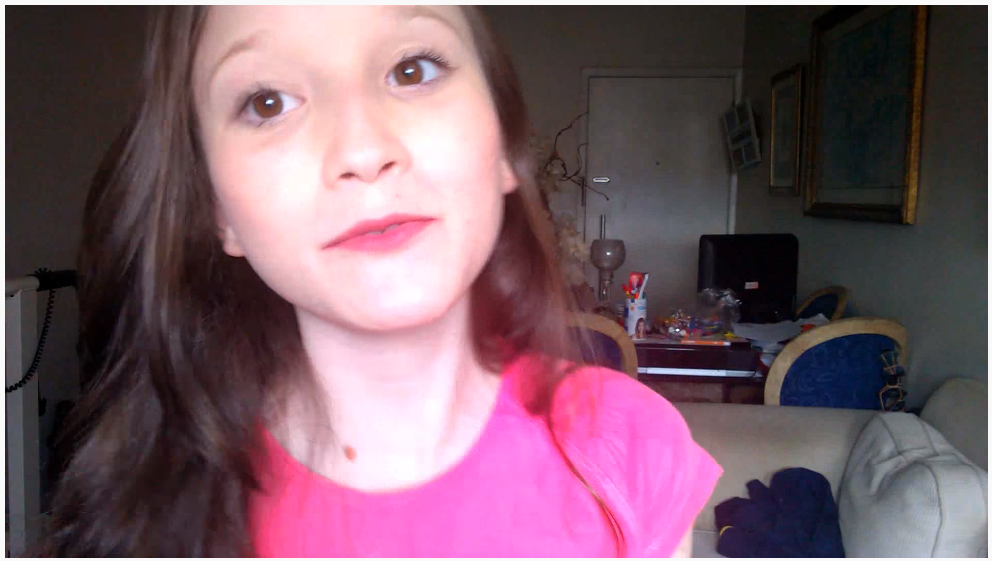
\includegraphics[width=0.7\linewidth]{fig/Zabetta-13-anos}
    \caption{vb}
    \label{fig:zabetta-13-anos}
\end{figure}


No vídeo \url{https://www.youtube.com/watch?v=QDMu3dTOoVI} ela brinca num desafio com cereja e chantily vemos que ela é a caçula de outros 3 irmãos. Aparentemente eles são muito amorosos um com outro.

No vídeo \url{https://www.youtube.com/watch?v=z0VjIP5AUAU} ela se permite mostrar alguns erros de gravação, mostrando um pouco dela como ela realmente é. Nesse vídeo mostra a interação com produtos que ela ganhou de aniversário. Fácil notar que tirando o HD e o PowerBank indutivo, todos os demais produtos são do universo feminino, maquiagem e beleza.



Em \url{https://www.youtube.com/watch?v=cH0fpW70ujY} ela faz algo muito típico de meninas no YouTube na idade dela: tutorial de maquilagem e como se vestir. É o jantar do ano novo de 2015, a falta do pai sugere que ela é filha de pais separados.

Vemos um exemplo de interação social no vídeo \url{https://www.youtube.com/watch?v=m46LF9b9NqU} referente a entrega de um prêmio para assinantes do canal. Tudo muito improvisado e rola uma certa timidez. Talvez fruto de não se preparar muito bem para a ocasião.

Um vídeo bem comum entre as meninas adolescentes youtubers é o react do seu material escolar no início do ano, como nesse vídeo referente ao começo do ano de 2015 em \url{https://www.youtube.com/watch?v=nXG0OKnmHpo}. O objetivo é claro, lançar tendências e mostrar seu stylelife\footnote{stylelife é estilo de vida.}. Curioso que o nível de exigência, talvez pela idade seja pouco.

Em \url{https://www.youtube.com/watch?v=N409jTfwMCg} ela se demonstra mais solta talvez por que achou engraçada a experiencia de andar horas seguidas no carro e precisou criar formas criativas e fofas de se livrar do tédio.

No vídeo \url{https://www.youtube.com/watch?v=wTd6gUh6BxI} comemoram 2 mil inscritos, o canal hoje tem 2,73 milhões.

No episódio \textbf{Meu celular foi destruído} \url{https://www.youtube.com/watch?v=-WGYaDwg0Fg} temos demonstrações de emoções como choro emocionado pelo celular novo que a mãe comprou e sua indignação pela quebra do celular. É nítido a frustração que ela não consegue falar o que aconteceu, provavelmente algo bobo que ela se envergonha. Importante verificar que existe uma consciência da mãe de que os jovens não podem ficar sem celular. A impressão que o aparelho é um "módulo de proteção" dos pais para com os filhos, já que permite comunicação instantânea com o rebento a qualquer hora. Pais mais neuróticos colocam rastreamento.

No episódio \textbf{\#Zabetta na cozinha - Bolo de Cenoura} \url{https://www.youtube.com/watch?v=pRk6TOCBrkY} ela mostra amigas de colégio, provavelmente do 9 ano do ensino fundamental. Ao contrário da protagonista as demais pessoas são muito tímidas, o que demonstra o contraste do preparo que a mesma faz para estar diante das câmeras.

No episódio Fale qualquer coisa \url{https://www.youtube.com/watch?v=G_XT9Ghtnpo} demonstra brincadeiras comuns entre youtubers jovens em busca de views por meio de humor pastelão. A interação com a mãe é engraçadíssimo.

Em \href{https://www.youtube.com/watch?v=WuJ_XpMSIws}{\textbf{\#VEDA - Tirando Dúvidas (MODELO,AGENCIA) (day 15)}} \url{https://www.youtube.com/watch?v=WuJ_XpMSIws} a mãe e a protagonista tiram dúvidas sobre a carreira de modelo, agenciamento. Existe uma nítida preocupação com os estudos e o futuro da menina. Tudo de forma bem transparente entre mãe e filha o que denuncia o cuidado da mãe com a filha caçula. Interessante a lista de documentos para permitir o trabalho da menor de idade em produtoras para gravação de um comercial.

A quantidade de inscritos chegou em 10 mil comemorados no vídeo \href{https://www.youtube.com/watch?v=KrqZuiVizzg}{\textbf{10.000 Inscritos \#VEDA (day 23 )}}. \url{https://www.youtube.com/watch?v=KrqZuiVizzg} onde a protagonista mostra depoimentos de fãs do próprio colégio dela. Interessante os depoimentos que mostram alguma hiperatividade e atitudes típicas de alunos do final do ensino fundamental. Detalhe do aluno que diz que não é gay embora pareça. Fiquei me perguntando dos esteriótipos e o bullying que ele vem sofrendo. Confesso que senti uma ponta de inveja e saudade da minha oitava série em 1988. A quantidade de amigos demonstrados foi muito alta. A sensação de pertencimento de um grupo é muito forte nesse vídeo. A comunidade de inscrito gira entre 10 e 17 anos em média pela aparência. A internet e as redes sociais diminuíram muito a distância entre ídolos e seus fãs, além de que não é mais necessário ter uma participação na TV para alavancar a carreira, sendo a divulgação boca a boca muito poderosa nesse meio.

O vídeo \href{https://www.youtube.com/watch?v=kRku3MWoG8A}{\textbf{Especial dia das mães}} \url{https://www.youtube.com/watch?v=kRku3MWoG8A} corrobora com a observação acima em que ela demonstra a emoção pela data especial.

No vídeo \href{https://www.youtube.com/watch?v=VRcU2faTZc4}{OBJETIVO - Vlog na Escola} \url{https://www.youtube.com/watch?v=VRcU2faTZc4} ela demonstra algumas cenas da escola em que ela estuda. Fascinante a vergonha diante da classe, a posição de destaque ou liderança perante a classe, mesmo que seja um amigo oculta.

Em \href{https://www.youtube.com/watch?v=KBkS6t55zEM}{MINHA MÃE FICOU MUITO BRAVA } \url{https://www.youtube.com/watch?v=KBkS6t55zEM} temos a oportunidade de ver bastidores da mãe editando os vídeos para o canal e uma trolagem da protagonista com a mãe usando um cabelo. Hilário e agonizante.

Nos episódios \href{https://www.youtube.com/watch?v=ezL9_lYwRWs}{Minha Rotina 2015 realidade na escola - TRAILER} \url{https://www.youtube.com/watch?v=ezL9_lYwRWs} e \href{https://www.youtube.com/watch?v=4cjxIiDx9yk}{\textbf{Vlog - Minha Rotina na Escola 2015}} \url{https://www.youtube.com/watch?v=4cjxIiDx9yk} temos oportunidade de ver algumas atividades que o colégio da protagonista desempenha com seus alunos. Experimentos de química, dança, entre outros. Além de encontros com fãs e amigas treslocadas no vídeo.

O canal comemora 1 ano com 30 mil inscrito com uma live \href{https://www.youtube.com/watch?v=Jp_d0ItrVS8}{aovivo Comemoração: 30k Inscritos e 1 Ano de Canal} \url{https://www.youtube.com/watch?v=Jp_d0ItrVS8}. A mãe comentou que ela deleta comentários de haters para não magoar a protagonista.




